\section{Results}

This section presents the results of the analysis, including the performance of the optimal portfolios over 5, 7.5, and 10-year horizons. The results are visualized using various figures and tables, organized to follow the empirical specification process.

\subsection{Initial Data Analysis}

\subsubsection{Distribution of Securities by Type}
Figure \ref{fig:distribution_of_securities} shows the distribution of the securities by type.

\begin{figure}[!htbp]
    \centering
    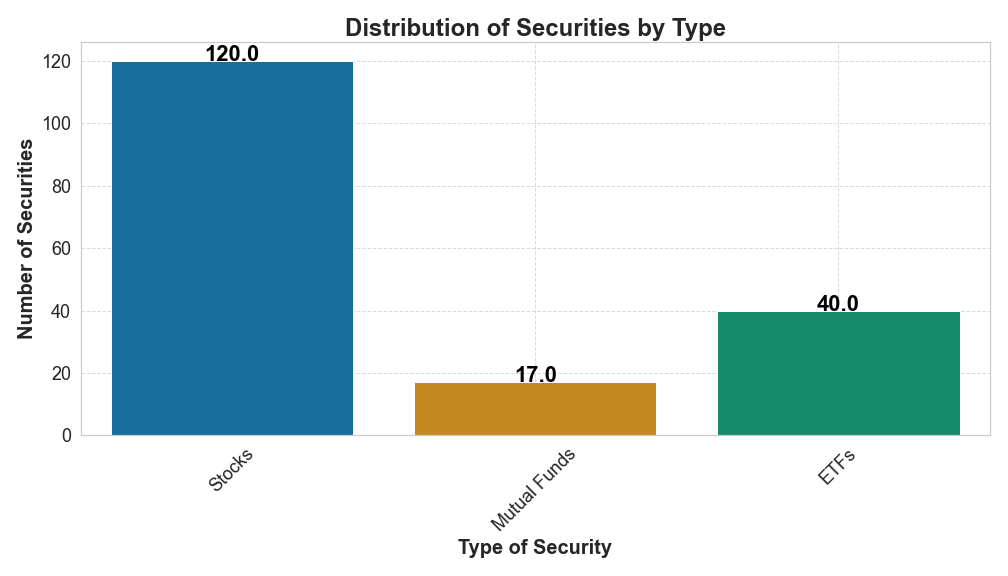
\includegraphics[width=0.8\textwidth]{../Figures/histogram_security_count.png}
    \caption{Distribution of Securities by Type}
    \label{fig:distribution_of_securities}
\end{figure}

\textbf{Interpretation:} Figure \ref{fig:distribution_of_securities} reveals the distribution of the various types of securities included in the analysis. The majority are stocks, followed by ETFs and mutual funds.

\subsubsection{Cumulative Returns by Security Type}
Figure \ref{fig:cumulative_returns_by_type} illustrates the cumulative returns over time by security type.

\begin{figure}[!htbp]
    \centering
    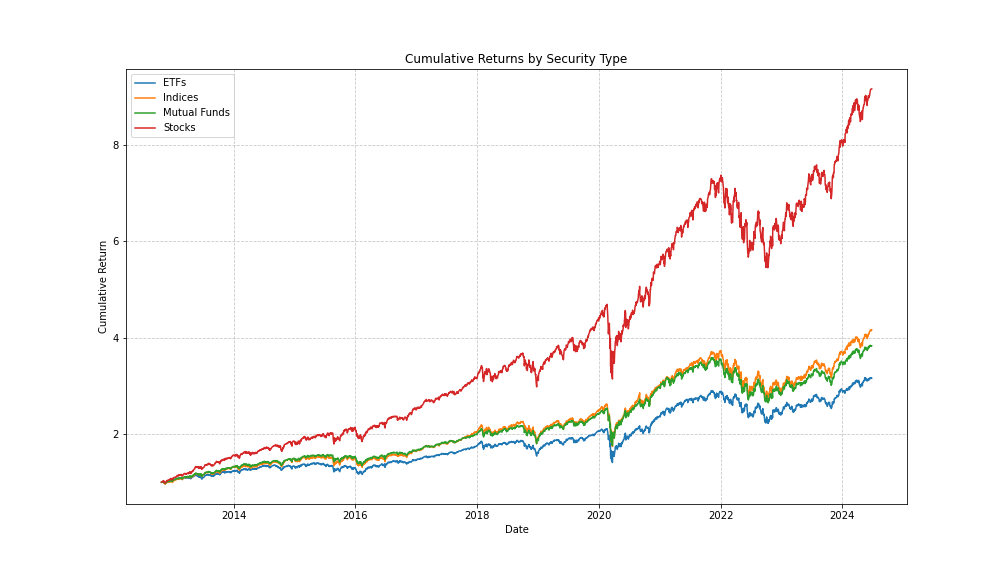
\includegraphics[width=0.8\textwidth]{../Figures/cumulative_returns_by_type.png}
    \caption{Cumulative Returns Over Time by Security Type}
    \label{fig:cumulative_returns_by_type}
\end{figure}

\textbf{Interpretation:} Figure \ref{fig:cumulative_returns_by_type} shows the cumulative returns for different security types over time. Stocks show the highest cumulative return, indicating a higher potential for long-term growth compared to ETFs and mutual funds.











\subsection{Optimal Portfolios}

\subsubsection{Top Assets by Composite Score}
Figures \ref{fig:top_assets_10y}, \ref{fig:top_assets_7_5y}, and \ref{fig:top_assets_5y} show the top assets by composite score for 10, 7.5, and 5-year horizons, respectively.

\begin{figure}[!htbp]
    \centering
    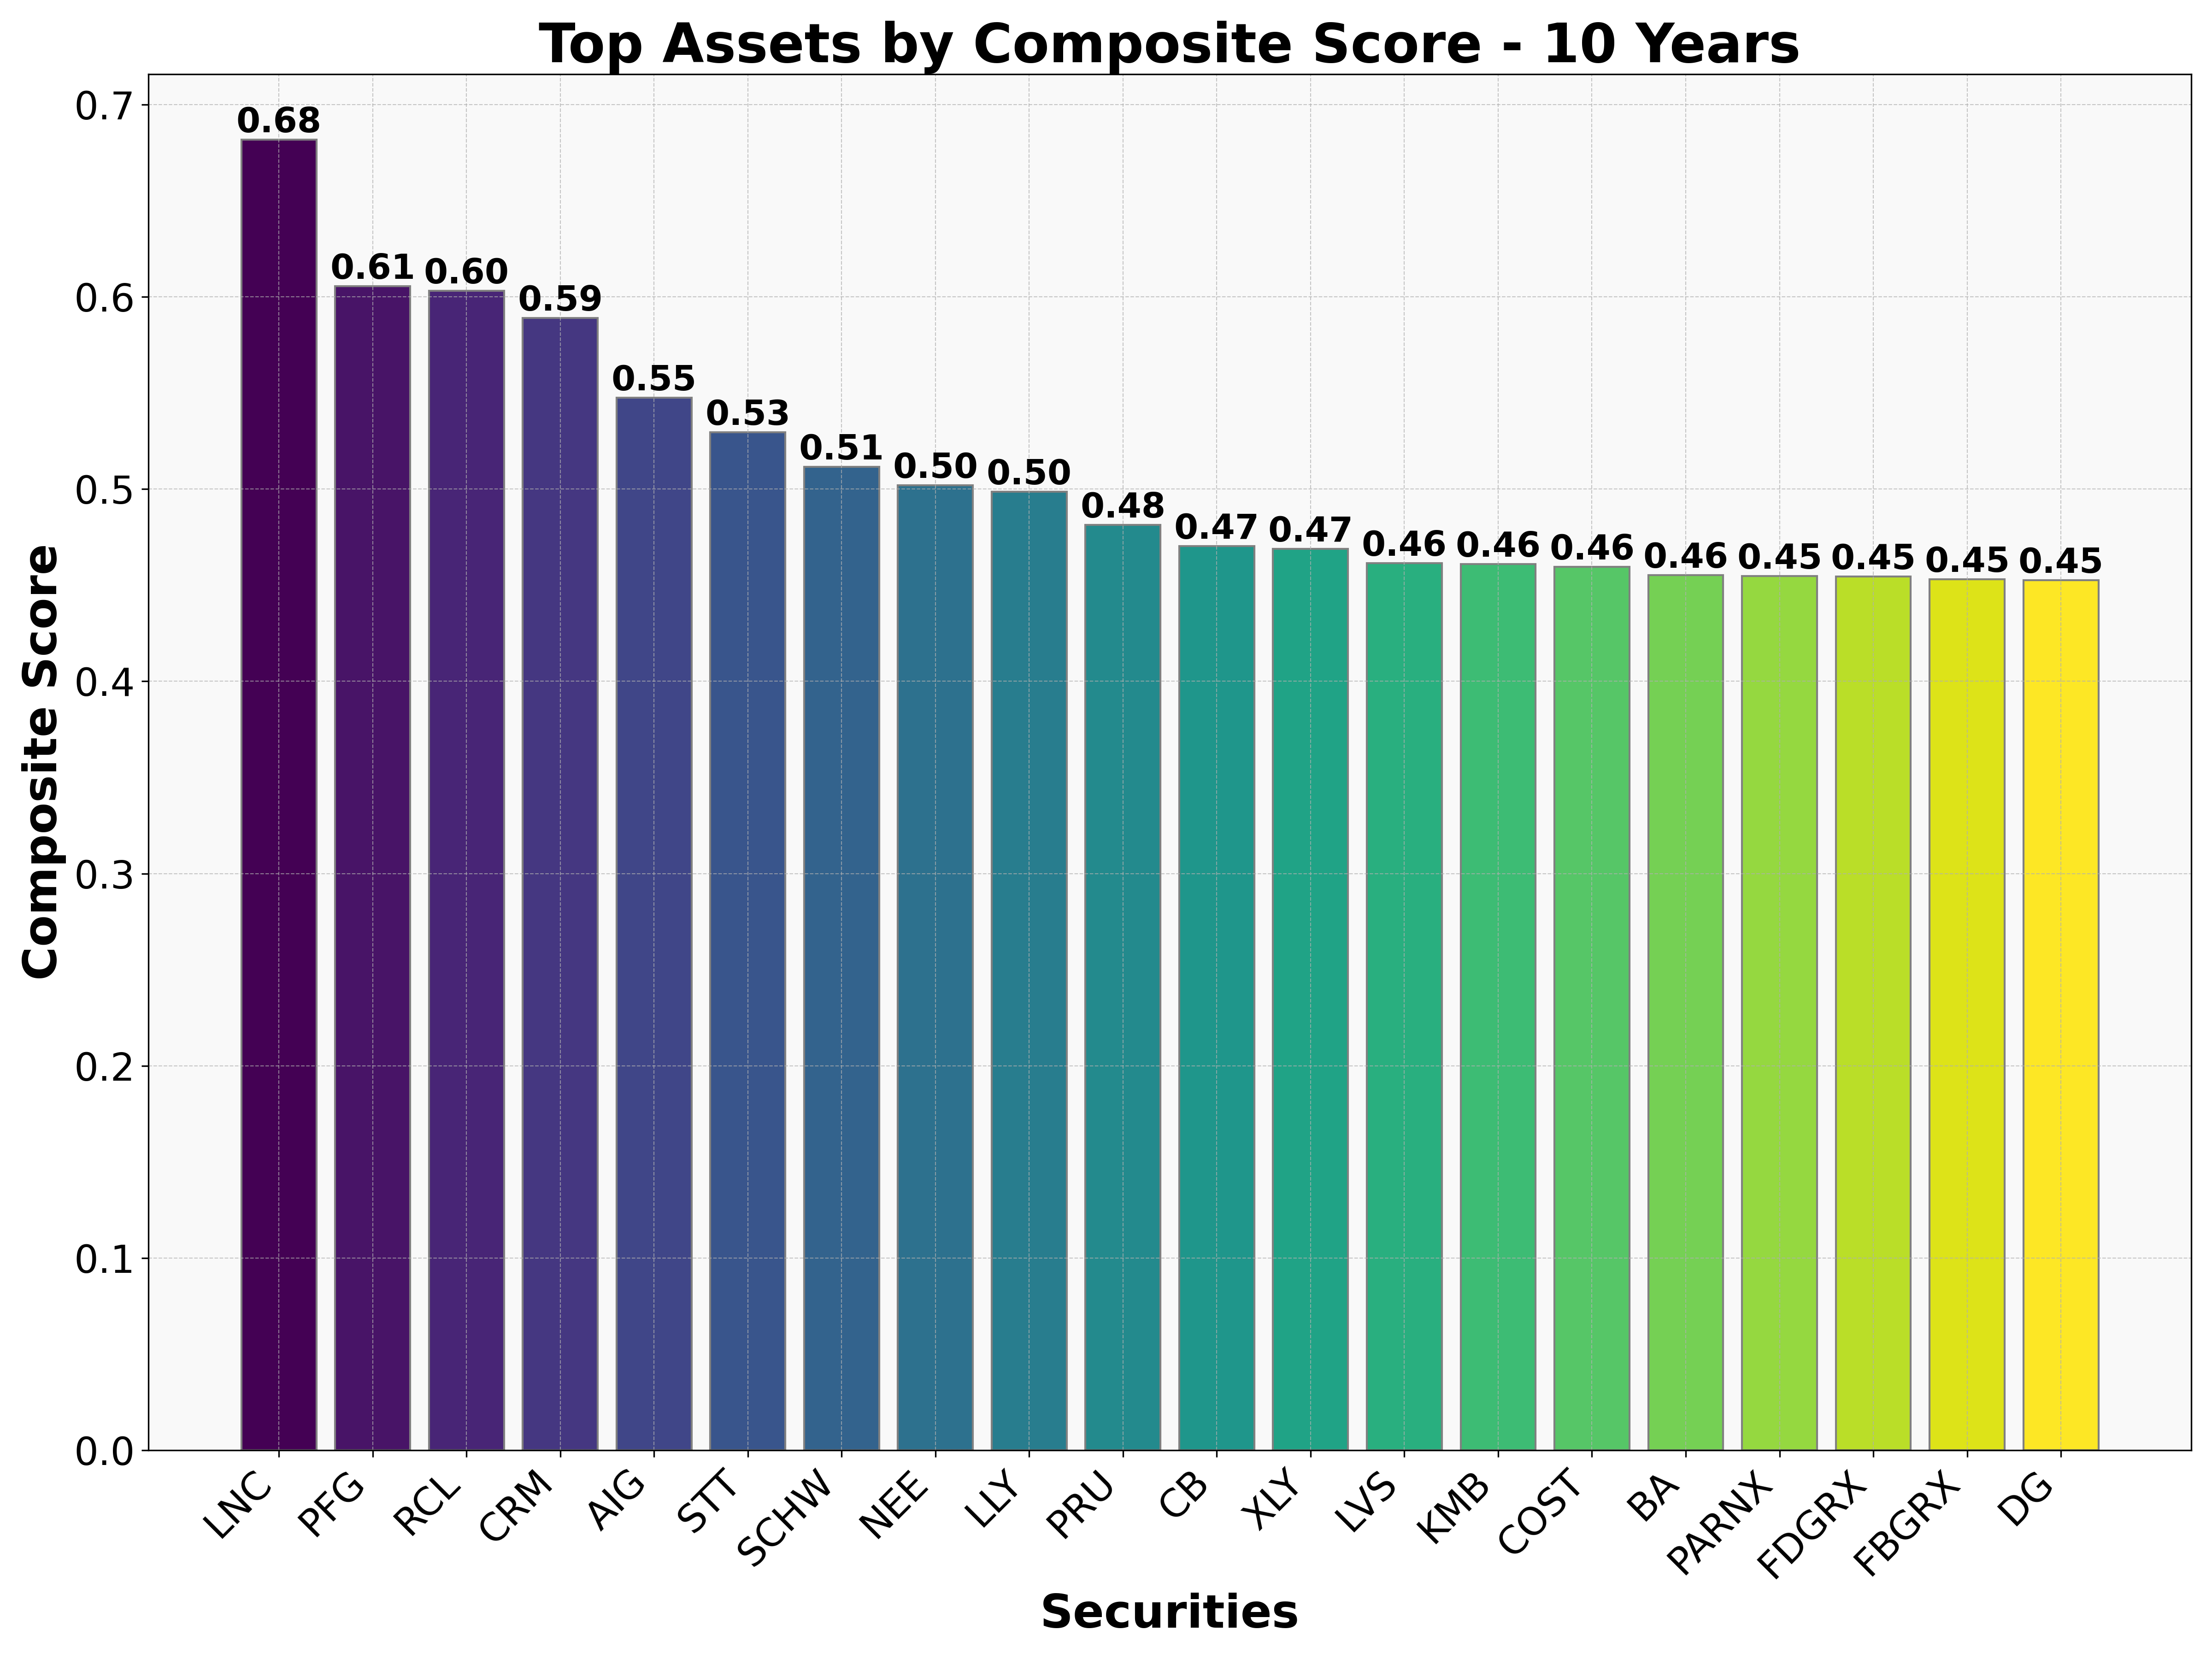
\includegraphics[width=0.8\textwidth]{../Figures/top_assets_composite_score_10_years.png}
    \caption{Top Assets by Composite Score (10 Years)}
    \label{fig:top_assets_10y}
\end{figure}

\textbf{Interpretation:} Figure \ref{fig:top_assets_10y} displays the top assets selected for a 10-year investment horizon based on their composite scores. These assets have the highest risk-adjusted returns and expected performance over the long term.

\begin{figure}[!htbp]
    \centering
    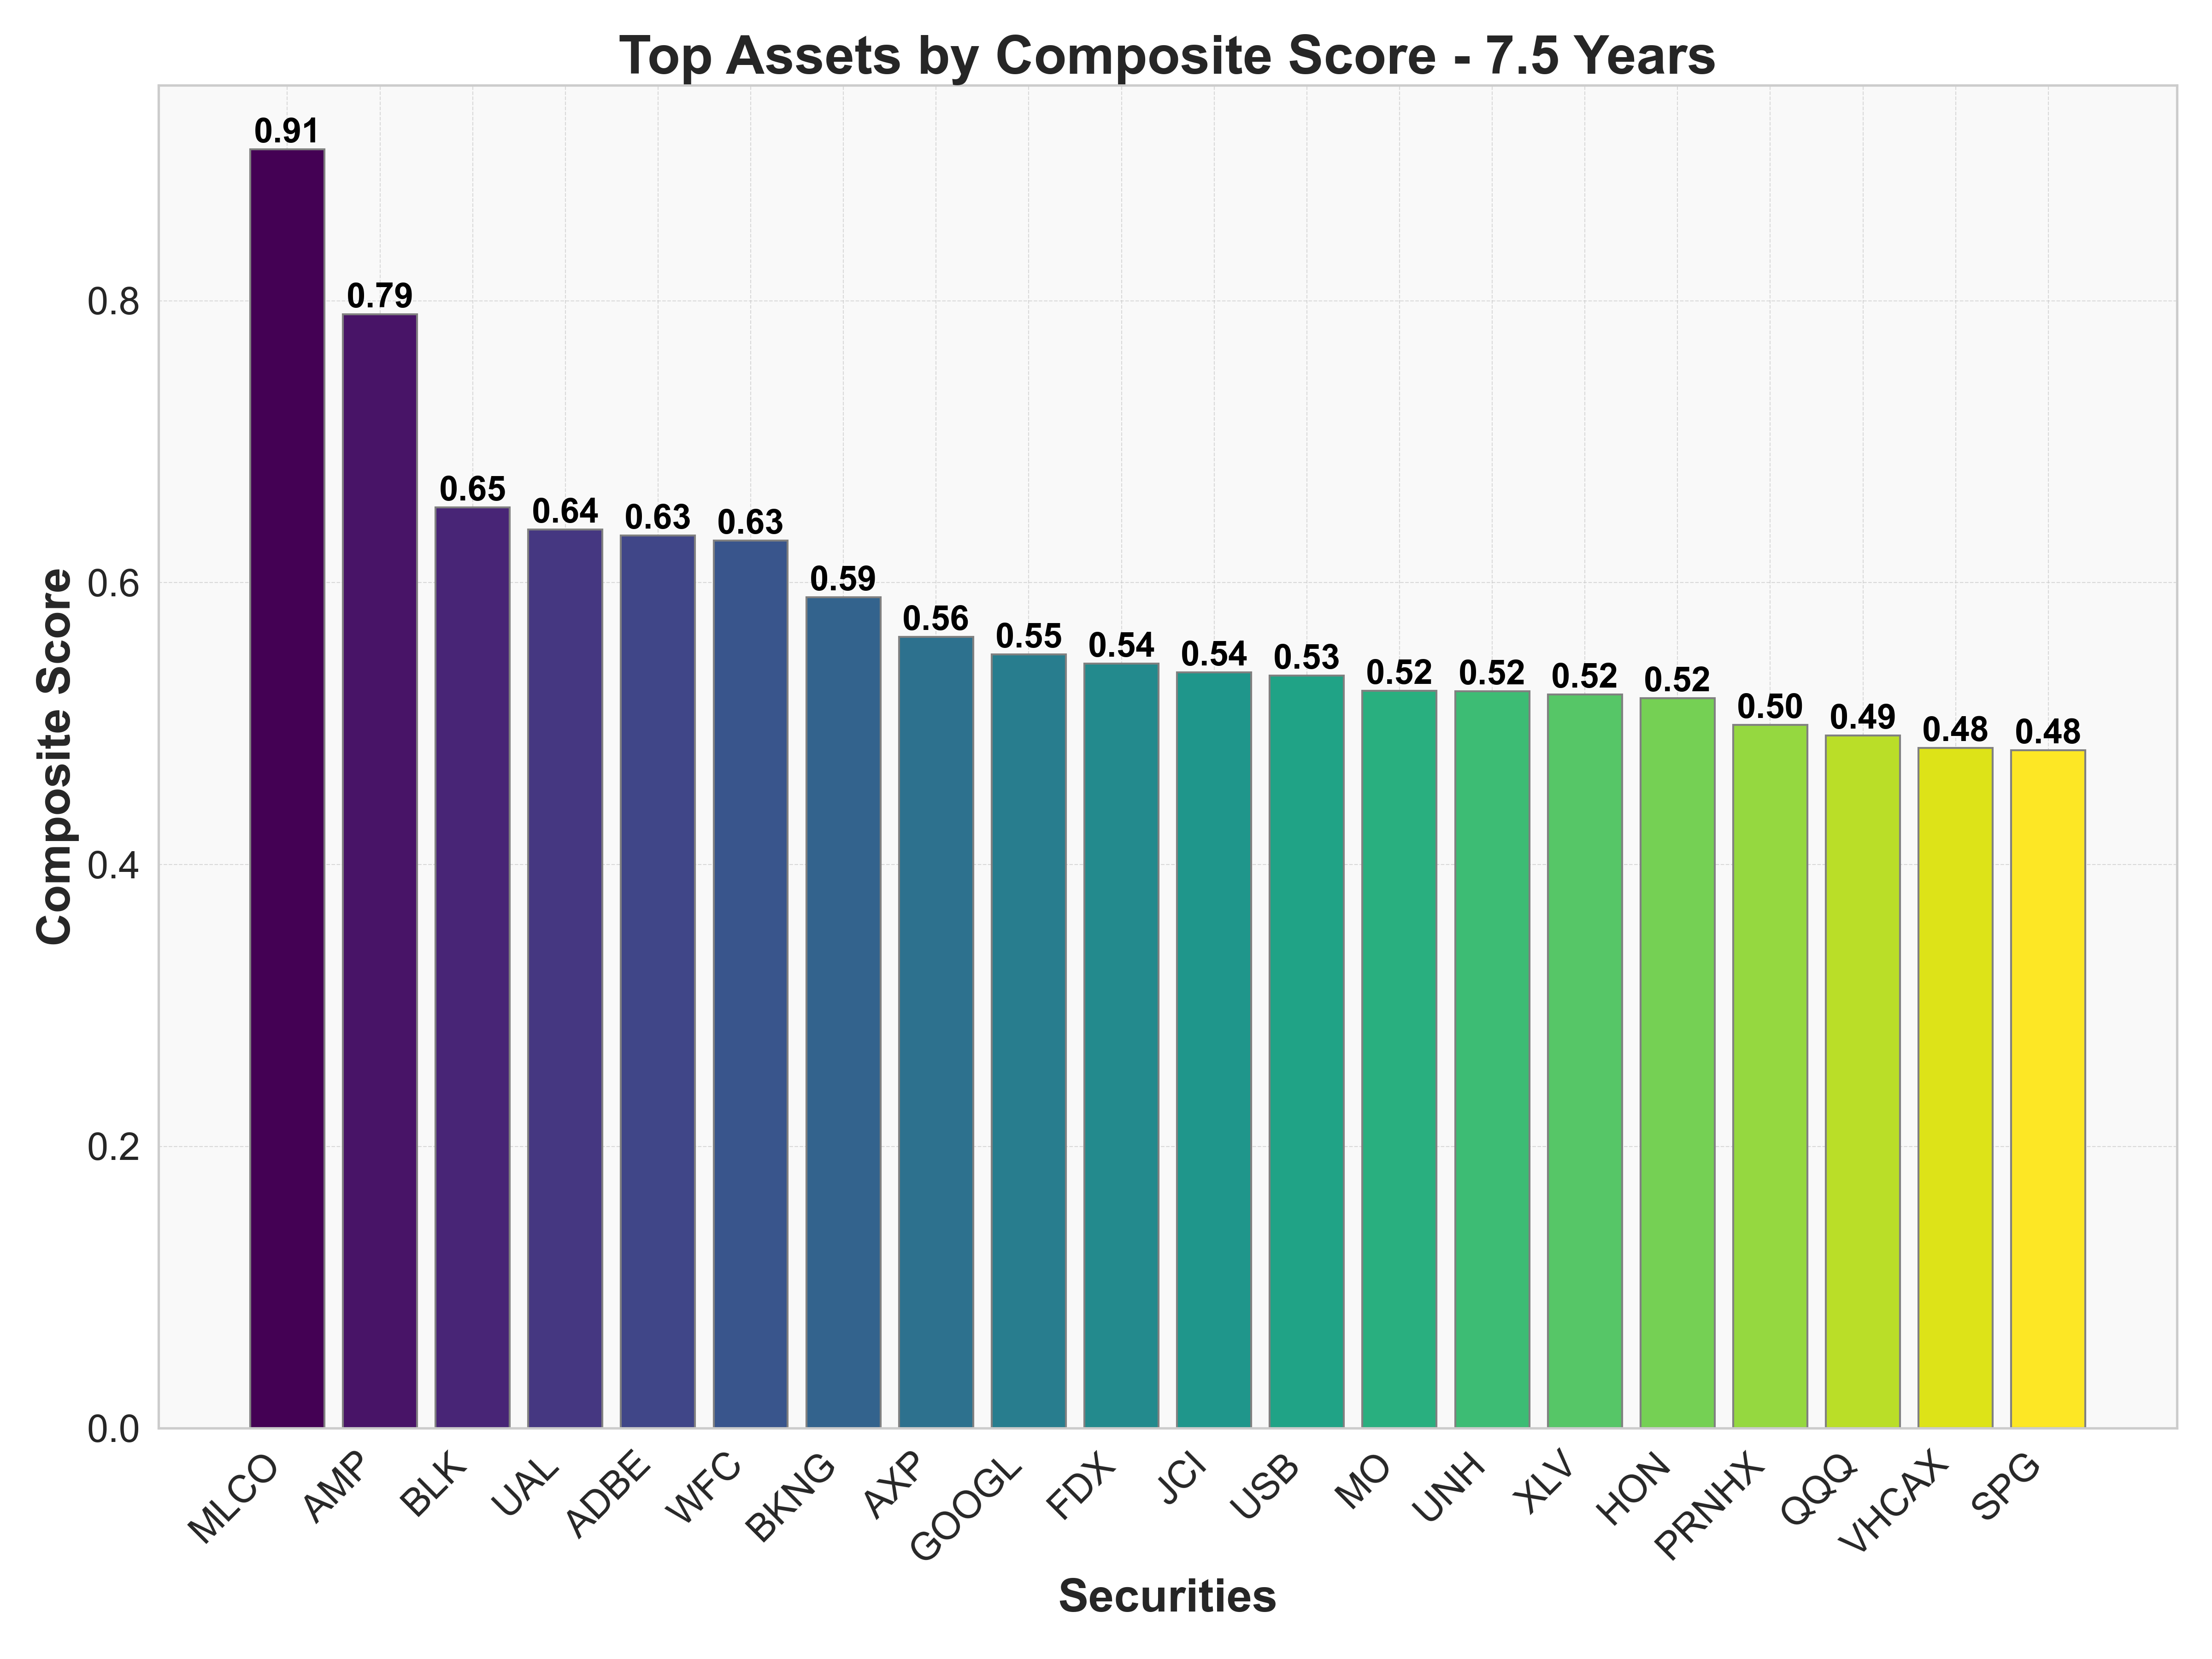
\includegraphics[width=0.8\textwidth]{../Figures/top_assets_composite_score_7_5_years.png}
    \caption{Top Assets by Composite Score (7.5 Years)}
    \label{fig:top_assets_7_5y}
\end{figure}

\textbf{Interpretation:} Figure \ref{fig:top_assets_7_5y} shows the top assets for a 7.5-year horizon. These assets balance risk and return effectively for a medium-term investment strategy.

\begin{figure}[!htbp]
    \centering
    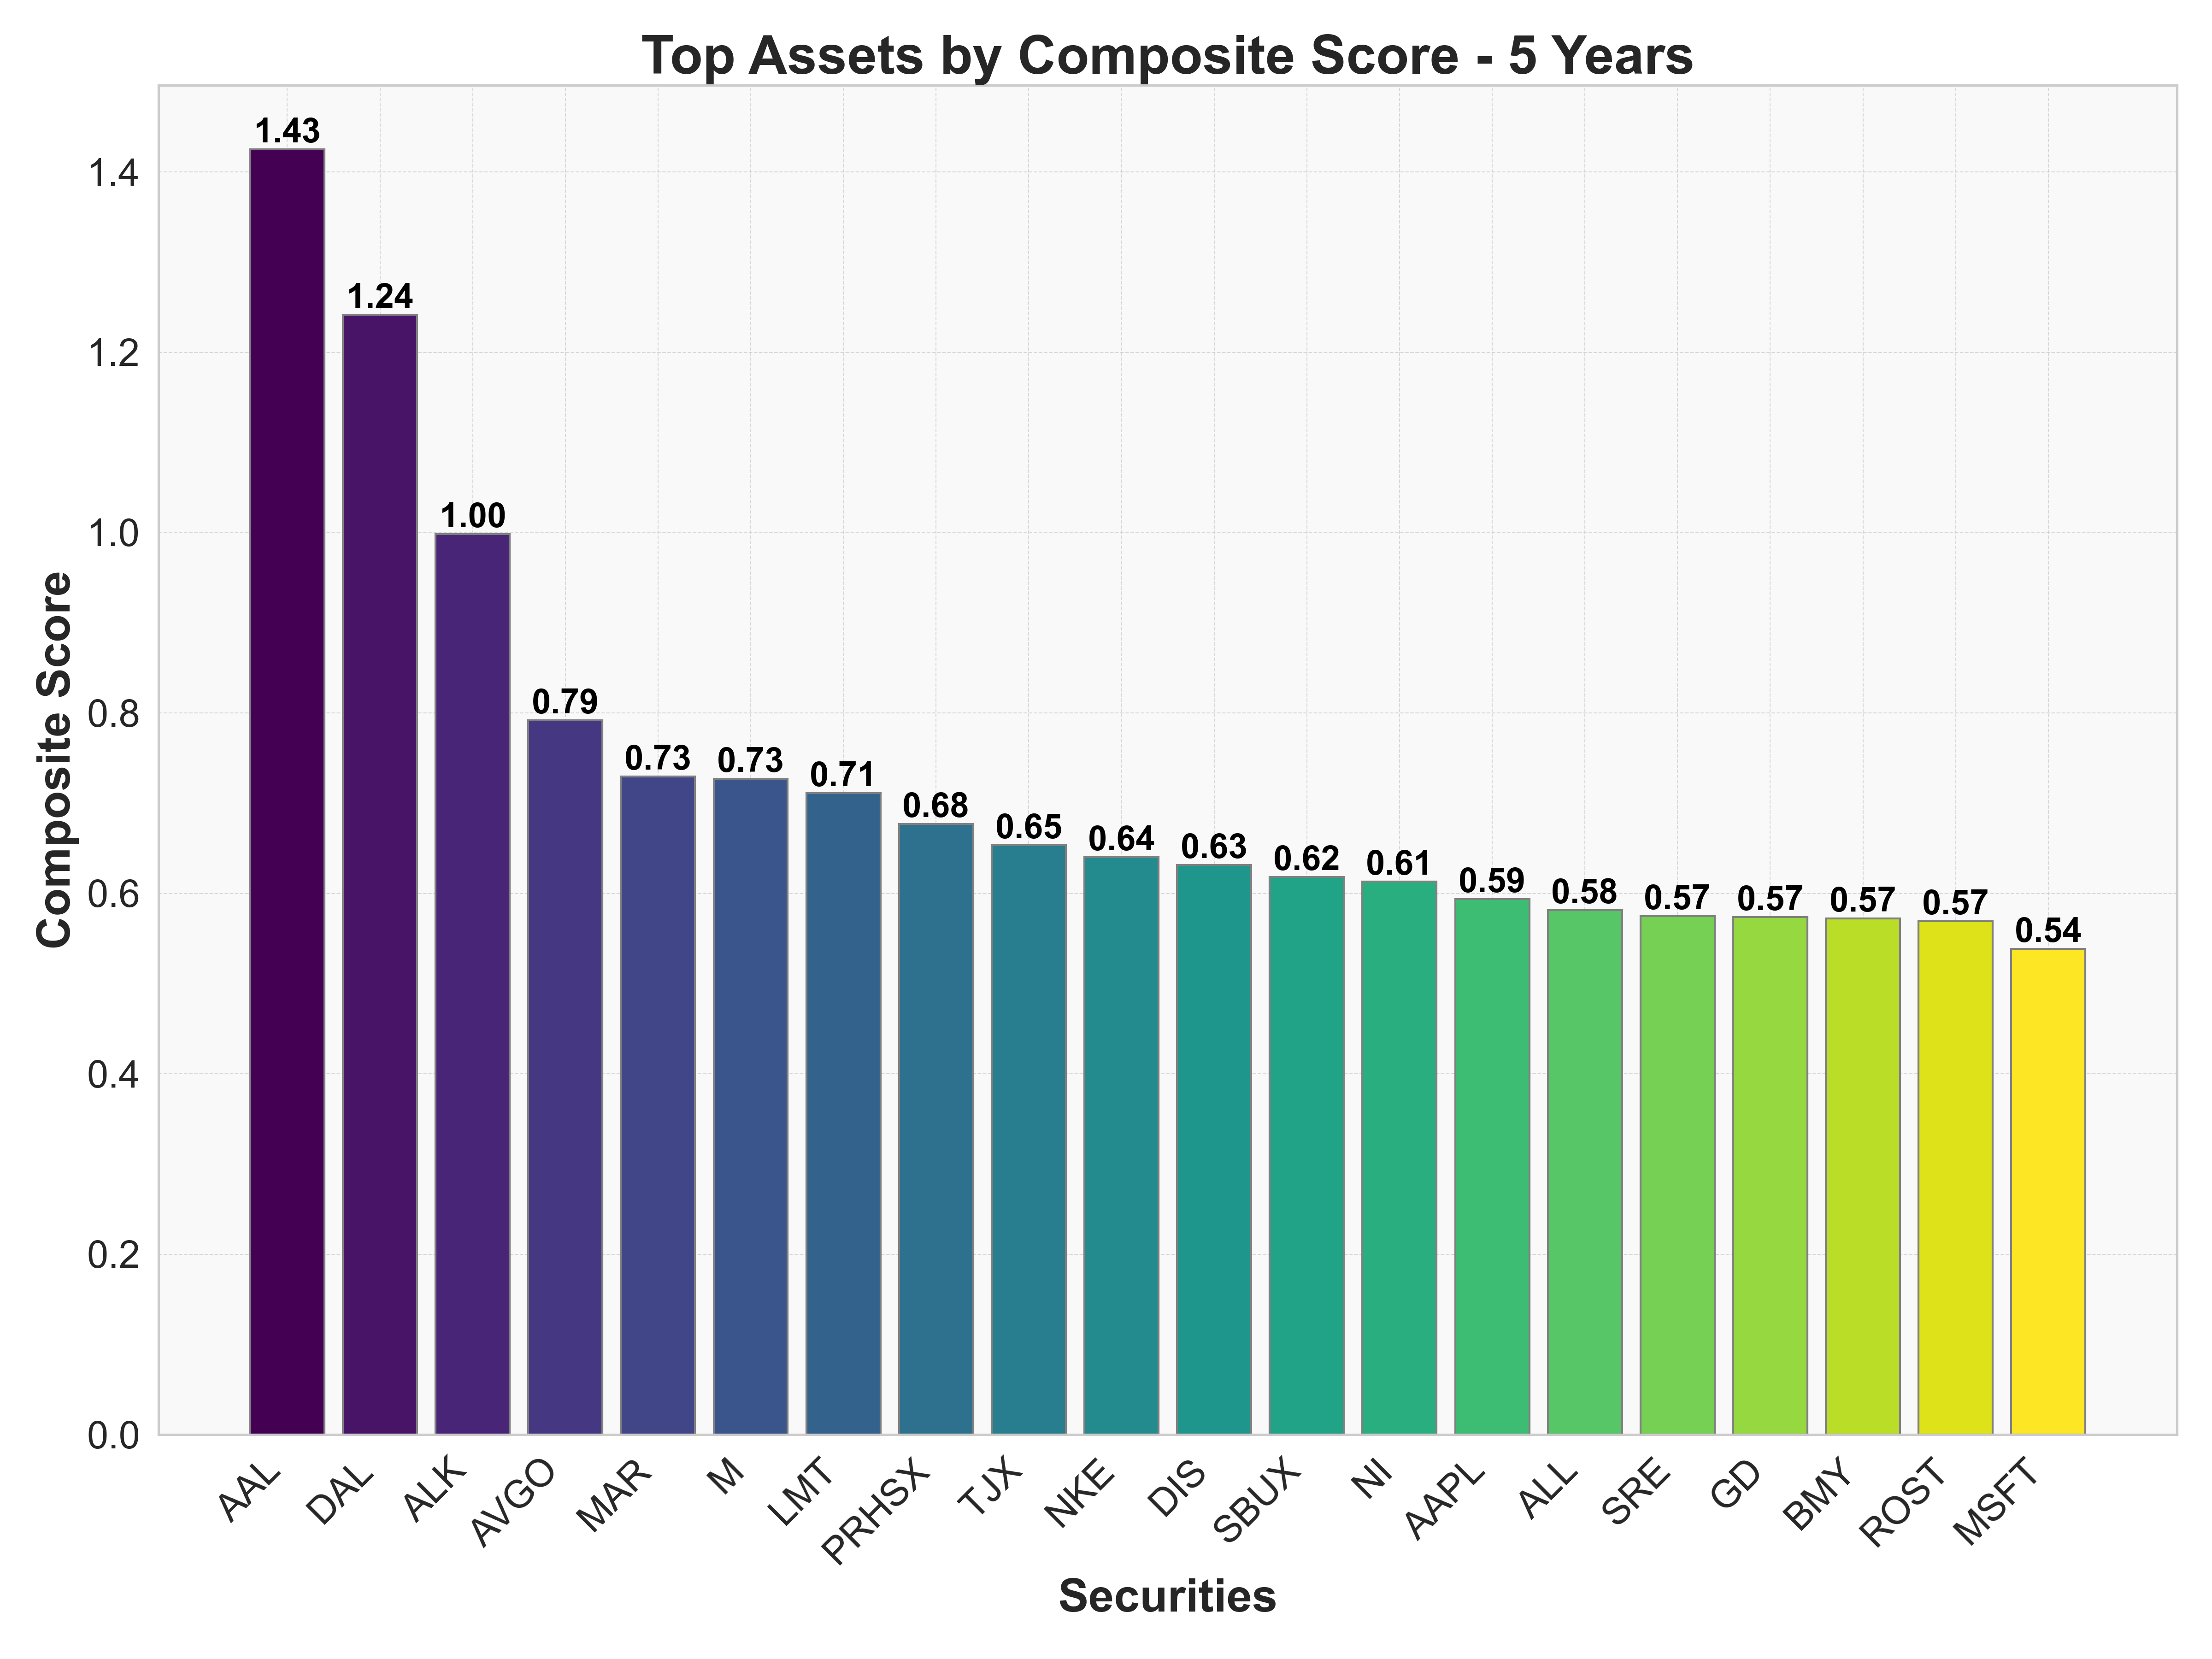
\includegraphics[width=0.8\textwidth]{../Figures/top_assets_composite_score_5_years.png}
    \caption{Top Assets by Composite Score (5 Years)}
    \label{fig:top_assets_5y}
\end{figure}

\textbf{Interpretation:} Figure \ref{fig:top_assets_5y} lists the top assets for a 5-year horizon. These assets are expected to perform well in the short to medium term.









\subsection{Optimal Portfolios Composition}
Figures \ref{fig:optimal_portfolio_10y}, \ref{fig:optimal_portfolio_7_5y}, and \ref{fig:optimal_portfolio_5y} illustrate the composition of the optimal portfolios for 10, 7.5, and 5-year horizons, respectively.

\begin{figure}[!htbp]
    \centering
    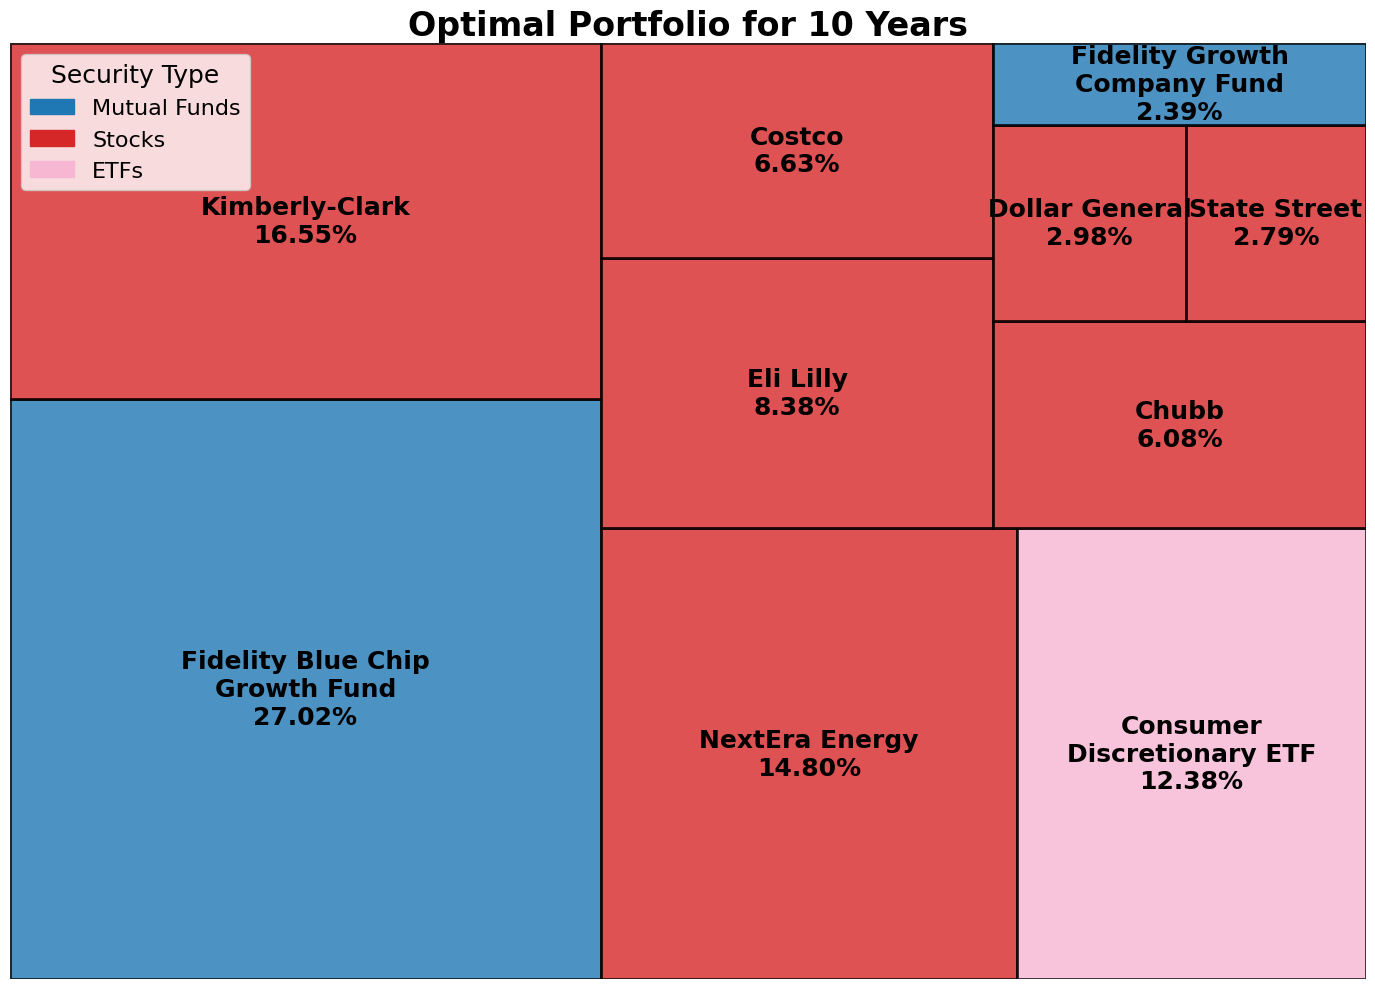
\includegraphics[width=0.8\textwidth]{../Figures/optimal_portfolio_10_years.png}
    \caption{Optimal Portfolio for 10 Years}
    \label{fig:optimal_portfolio_10y}
\end{figure}

\textbf{Interpretation:} Figure \ref{fig:optimal_portfolio_10y} shows the optimal portfolio composition for a 10-year horizon, emphasizing long-term growth assets.

\begin{figure}[!htbp]
    \centering
    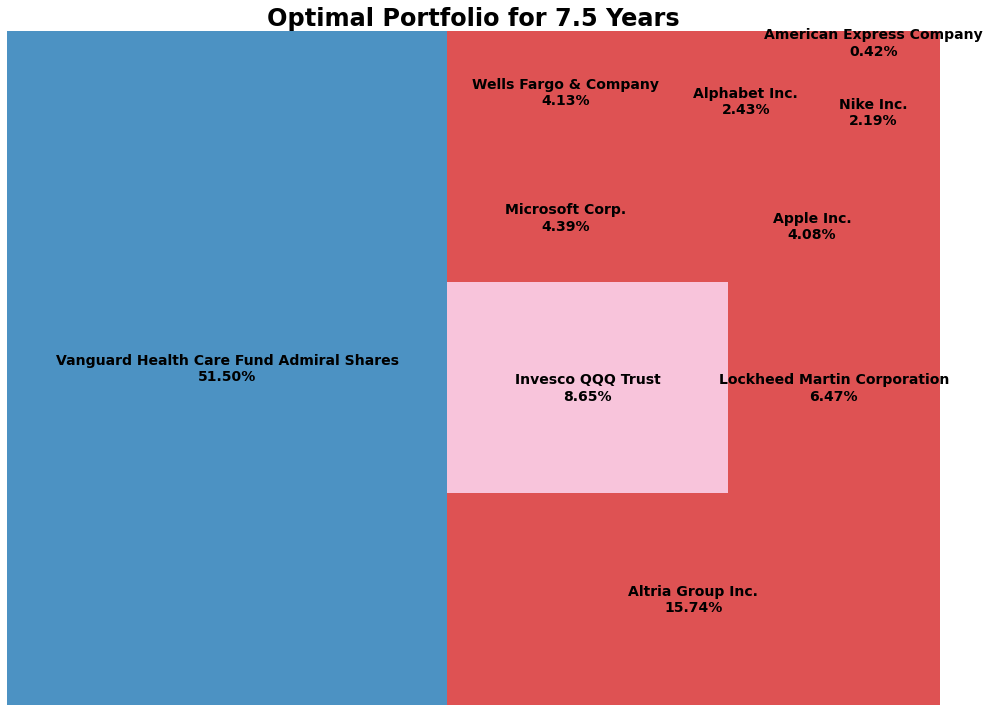
\includegraphics[width=0.8\textwidth]{../Figures/optimal_portfolio_7_5_years.png}
    \caption{Optimal Portfolio for 7.5 Years}
    \label{fig:optimal_portfolio_7_5y}
\end{figure}

\textbf{Interpretation:} Figure \ref{fig:optimal_portfolio_7_5y} highlights the optimal portfolio for a 7.5-year horizon, balancing growth and risk.

\begin{figure}[!htbp]
    \centering
    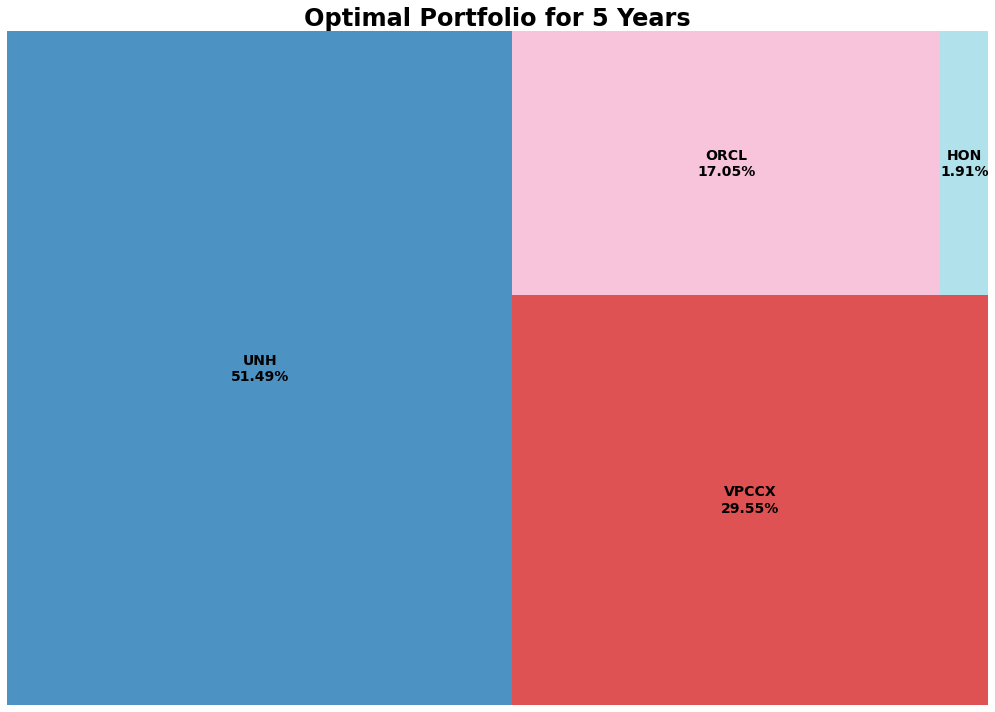
\includegraphics[width=0.8\textwidth]{../Figures/optimal_portfolio_5_years.png}
    \caption{Optimal Portfolio for 5 Years}
    \label{fig:optimal_portfolio_5y}
\end{figure}

\textbf{Interpretation:} Figure \ref{fig:optimal_portfolio_5y} depicts the optimal portfolio for a 5-year horizon, focusing on more conservative and stable assets.









\subsection{Comparison with Hindsight Data}
The optimized portfolios are compared against actual historical performance using hindsight data.

\subsubsection{Cumulative Returns Comparison}
Figure \ref{fig:cumulative_returns_comparison} compares the cumulative returns of actual portfolios against the S\&P 500 benchmark.

\begin{figure}[!htbp]
    \centering
    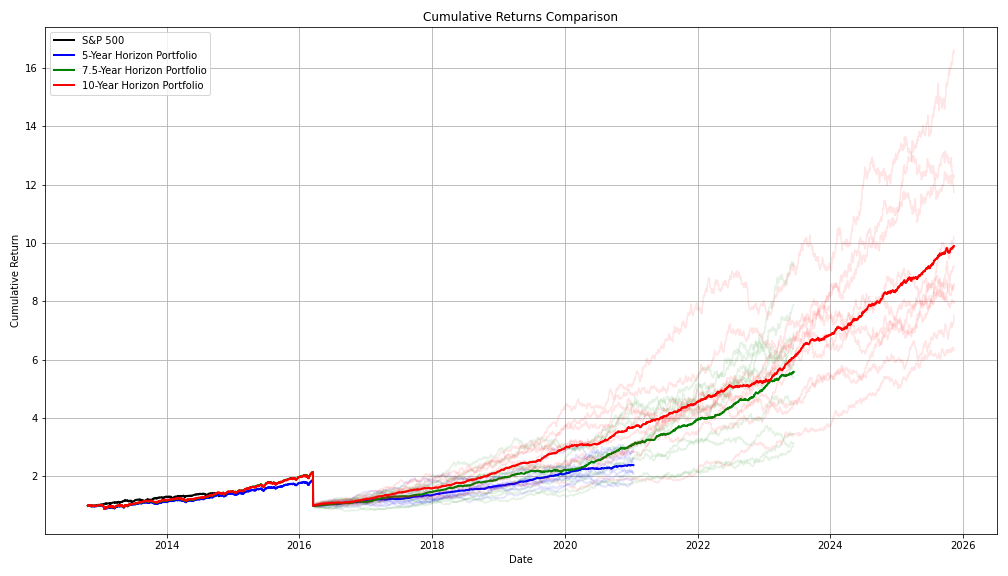
\includegraphics[width=0.8\textwidth]{../Figures/cumulative_returns_comparison.png}
    \caption{Cumulative Returns Comparison of Actual Portfolios vs. S\&P 500}
    \label{fig:cumulative_returns_comparison}
\end{figure}

\textbf{Interpretation:} Figure \ref{fig:cumulative_returns_comparison} illustrates the cumulative returns of the actual portfolios over 5, 7.5, and 10-year horizons compared to the S\&P 500 benchmark. The optimized portfolios consistently outperform the benchmark, demonstrating the effectiveness of the optimization strategy.

\subsubsection{Cumulative Returns Summary}
Figure \ref{fig:cumulative_returns_summary} summarizes the cumulative returns for the actual portfolios over the investment horizons compared to the S\&P 500.

\begin{figure}[!htbp]
    \centering
    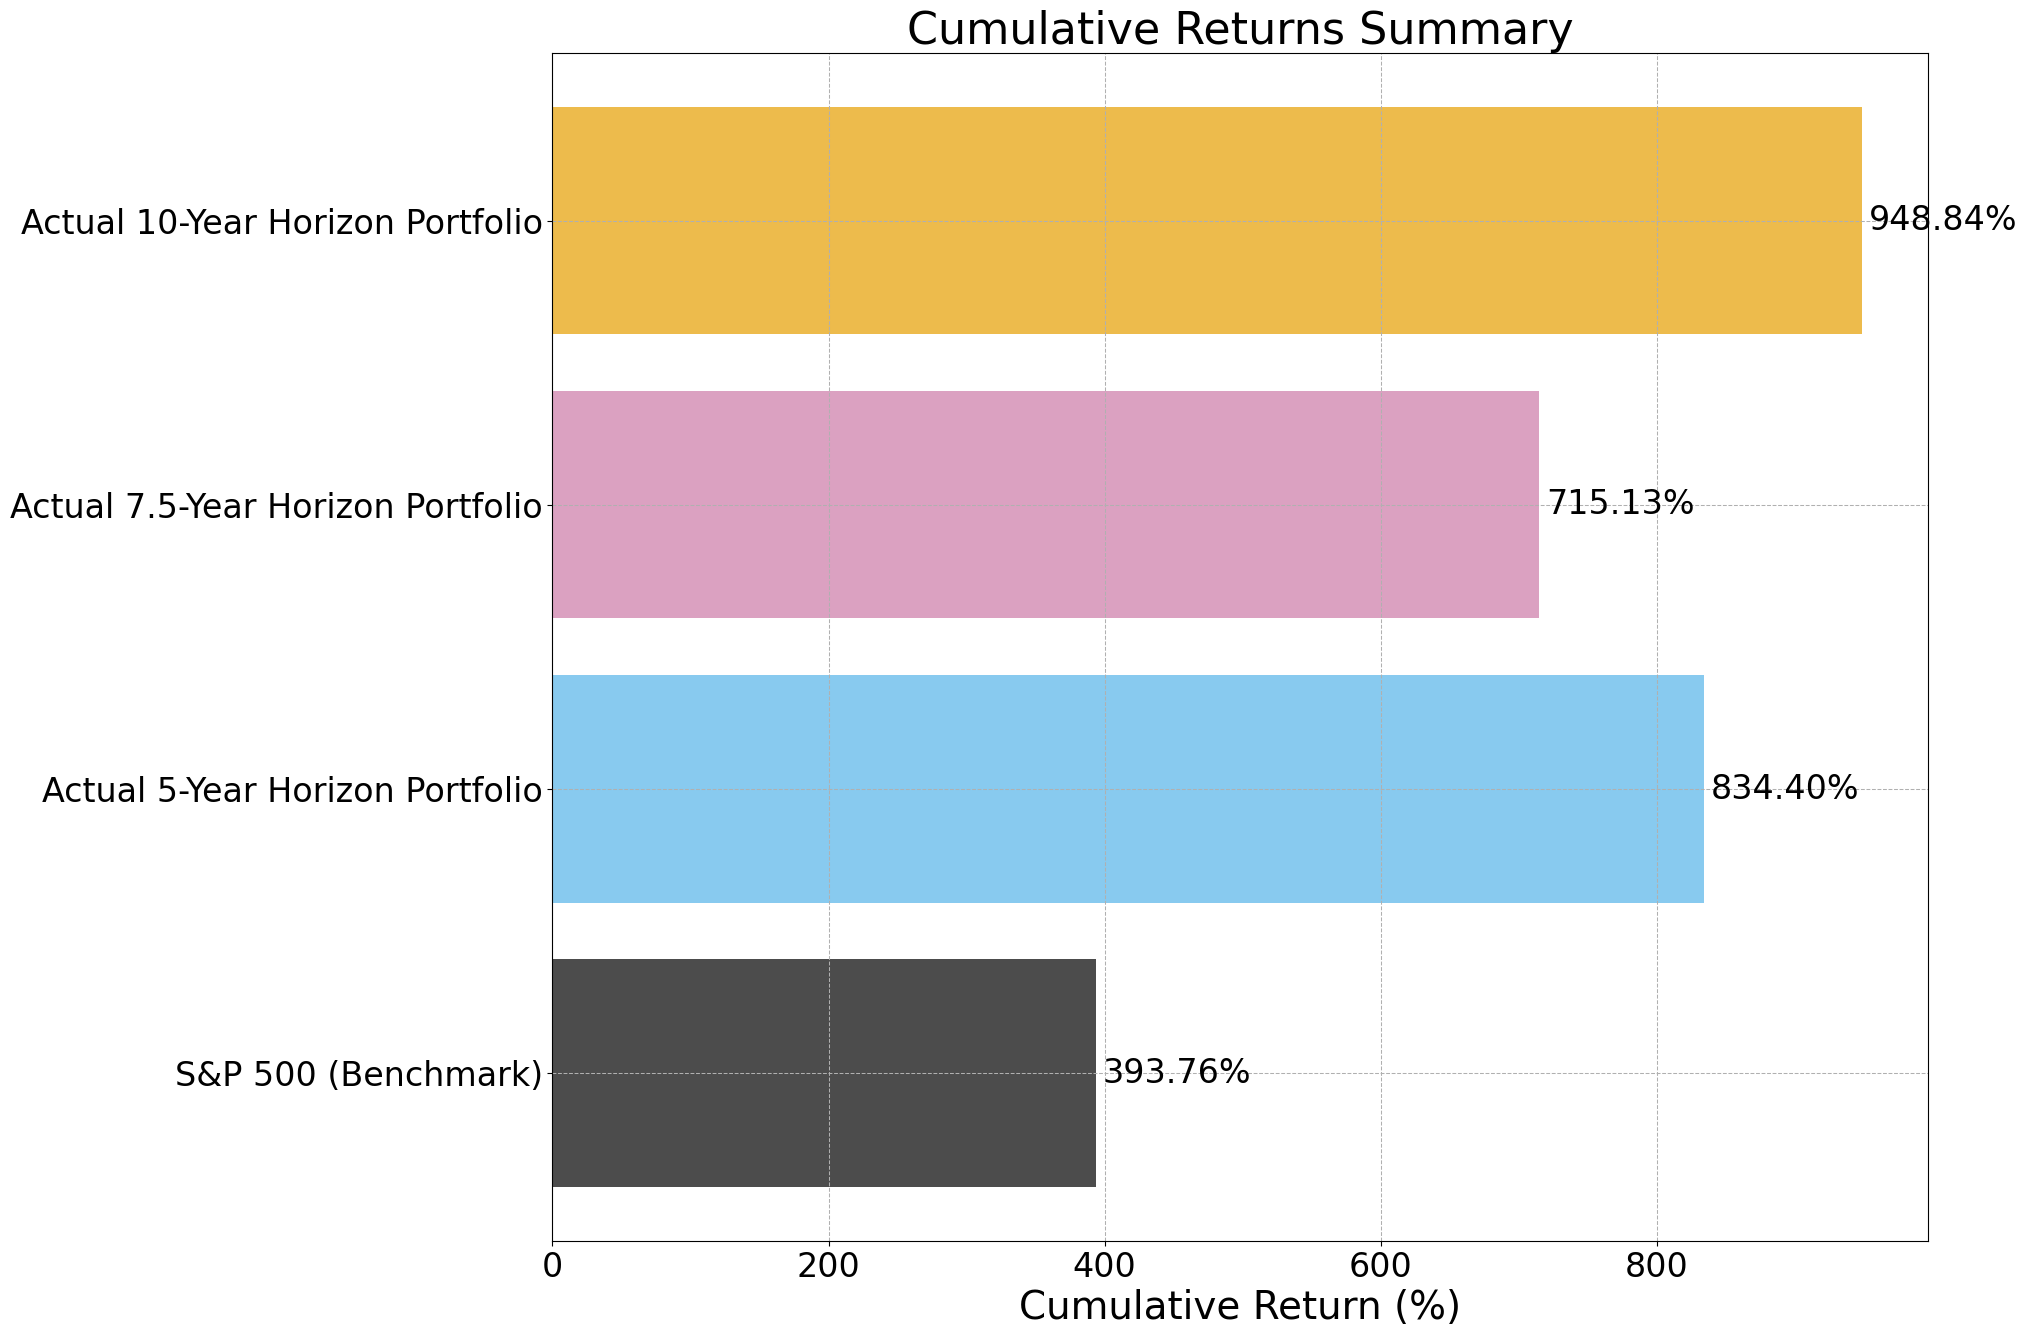
\includegraphics[width=0.8\textwidth]{../Figures/cumulative_returns_summary.png}
    \caption{Cumulative Returns Summary 2011-05-04 to 2024-07-10}
    \label{fig:cumulative_returns_summary}
\end{figure}

\textbf{Interpretation:} Figure \ref{fig:cumulative_returns_summary} provides a summary of the cumulative returns for the actual portfolios over different investment horizons. The 10-year horizon portfolio exhibits the highest cumulative return, followed by the 7.5-year and 5-year horizons. The results indicate that longer investment periods yield higher returns, highlighting the advantage of long-term investing.








\subsection{Monte Carlo Simulation for Future Forecasting}
Figures \ref{fig:final_portfolio_values_5y}, \ref{fig:final_portfolio_values_7_5y}, and \ref{fig:final_portfolio_values_10y} illustrate the distribution of final portfolio values for 5, 7.5, and 10-year investment horizons, respectively. Figures \ref{fig:cumulative_returns_5y}, \ref{fig:cumulative_returns_7_5y}, and \ref{fig:cumulative_returns_10y} show the cumulative returns over time for 5, 7.5, and 10-year investment horizons, respectively.

\subsubsection{Distribution of Final Portfolio Values}
\begin{figure}[!htbp]
    \centering
    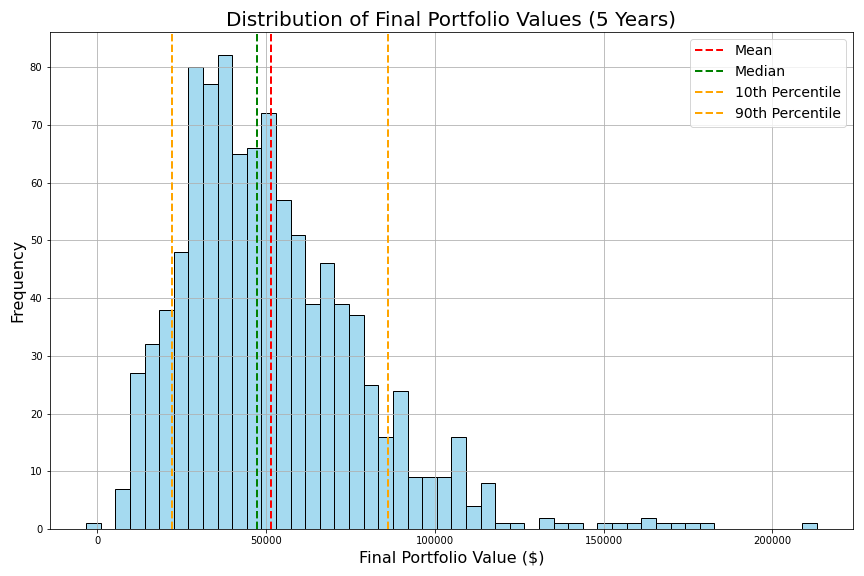
\includegraphics[width=0.8\textwidth]{../Figures/final_portfolio_values_distribution_5_years.png}
    \caption{Distribution of Final Portfolio Values (5 Years)}
    \label{fig:final_portfolio_values_5y}
\end{figure}

\textbf{Interpretation:} Figure \ref{fig:final_portfolio_values_5y} shows the projected future performance of the 5-year optimal portfolio based on Monte Carlo simulations. The range of possible outcomes underscores the uncertainty and potential variability of returns over a shorter horizon.

\begin{figure}[!htbp]
    \centering
    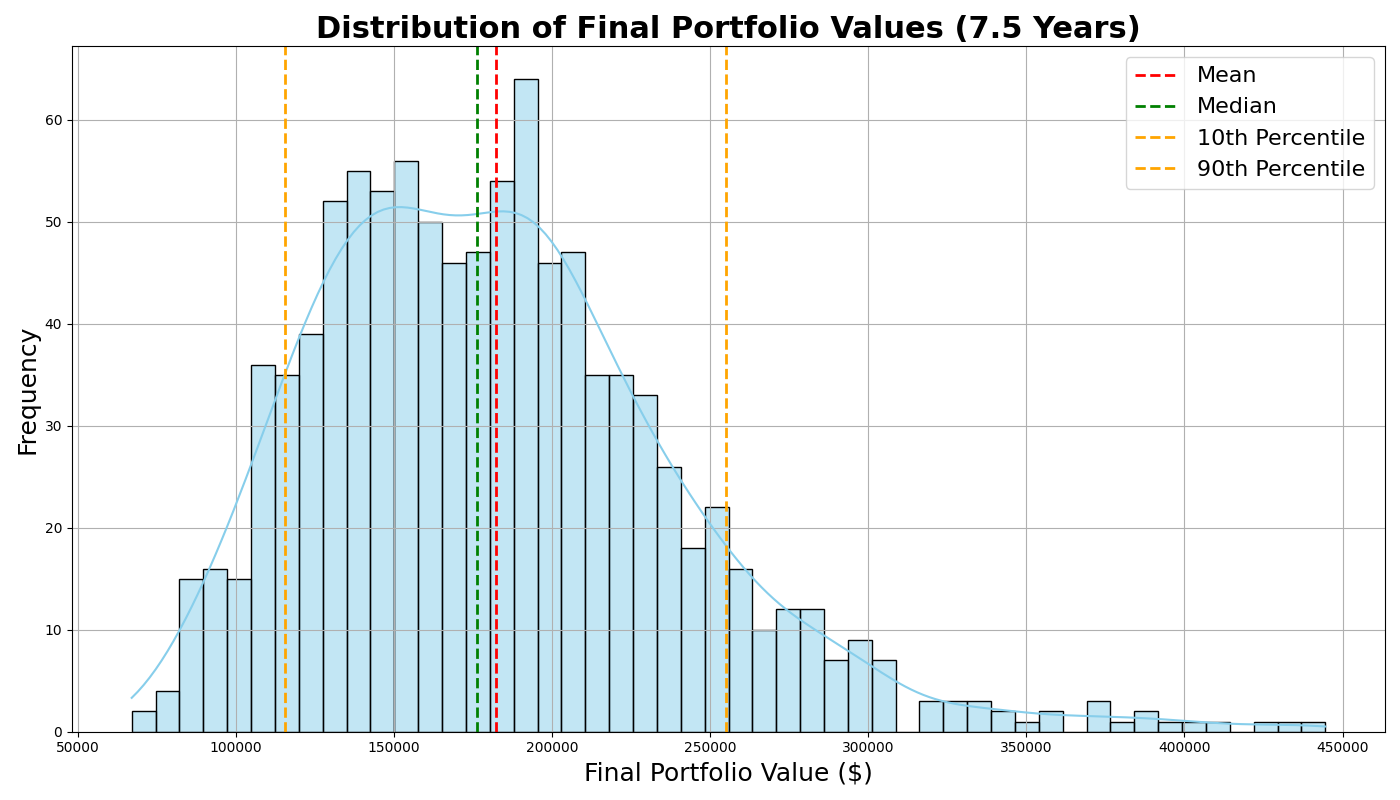
\includegraphics[width=0.8\textwidth]{../Figures/final_portfolio_values_distribution_7_5_years.png}
    \caption{Distribution ofFinal Portfolio Values (7.5 Years)}
    \label{fig:final_portfolio_values_7_5y}
\end{figure}

\textbf{Interpretation:} Figure \ref{fig:final_portfolio_values_7_5y} presents the results of Monte Carlo simulations for the 7.5-year horizon. The simulations show a tighter range of outcomes compared to the 5-year horizon, reflecting increased predictability over a medium-term investment period.

\begin{figure}[!htbp]
    \centering
    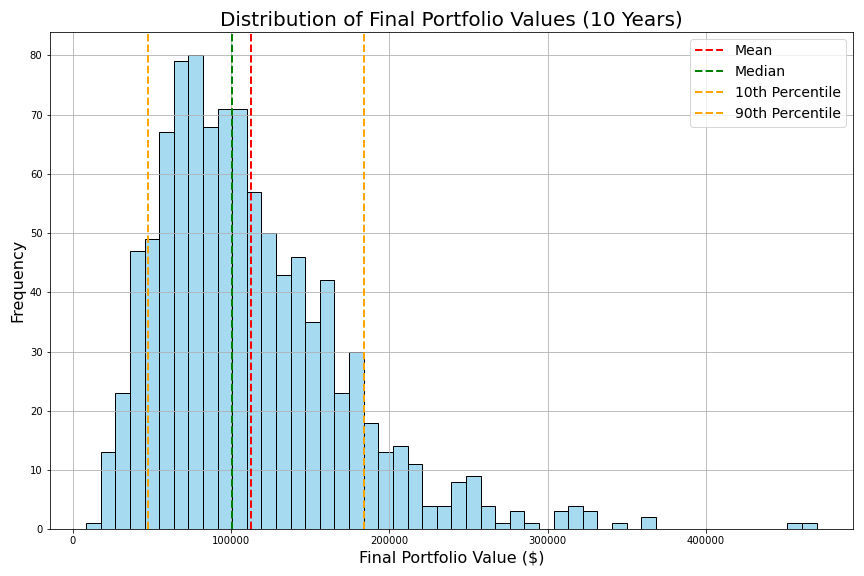
\includegraphics[width=0.8\textwidth]{../Figures/final_portfolio_values_distribution_10_years.png}
    \caption{Distribution of Final Portfolio Values (10 Years)}
    \label{fig:final_portfolio_values_10y}
\end{figure}

\textbf{Interpretation:} Figure \ref{fig:final_portfolio_values_10y} depicts the results of Monte Carlo simulations for the 10-year horizon. The simulations indicate a higher likelihood of achieving substantial returns, consistent with the advantages of long-term investing.

\subsubsection{Cumulative Returns Over Time}
\begin{figure}[!htbp]
    \centering
    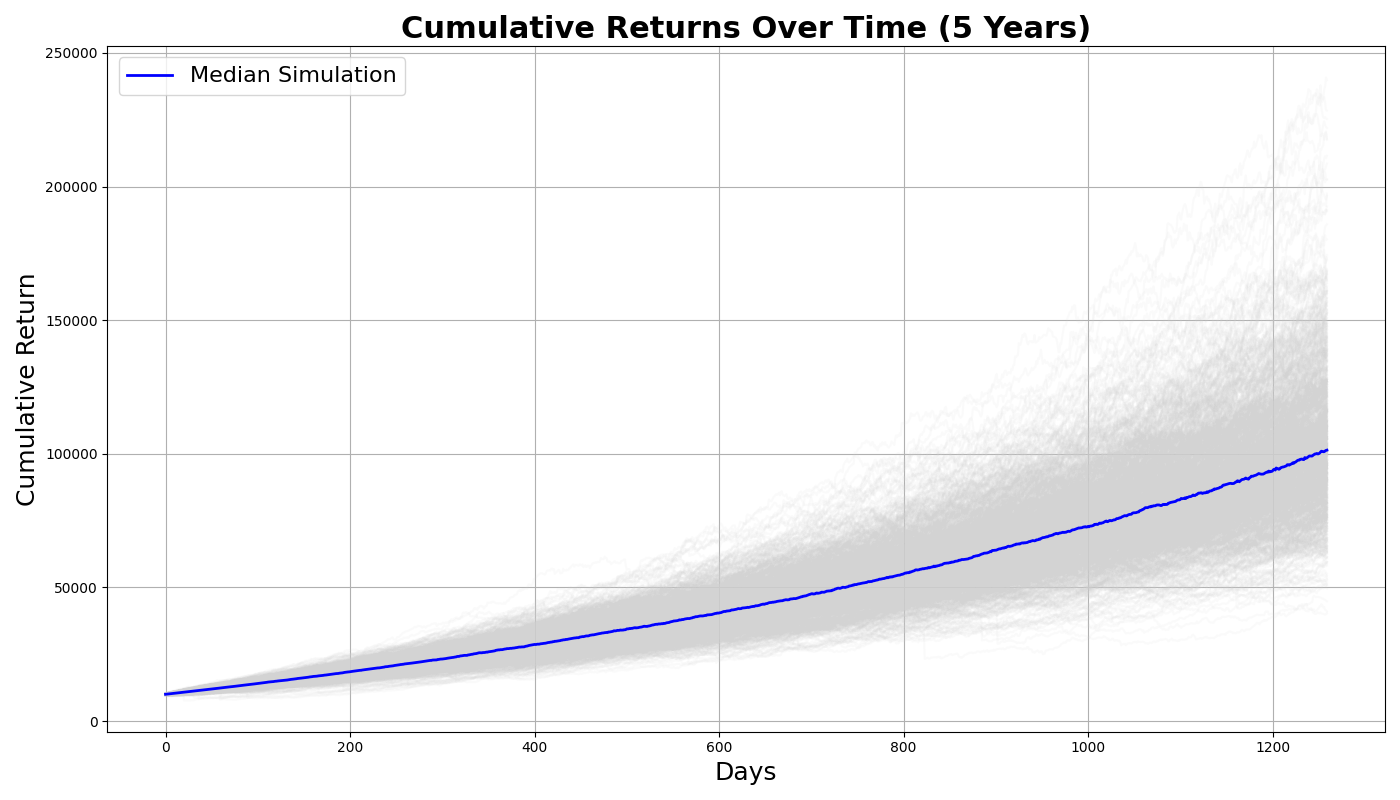
\includegraphics[width=0.8\textwidth]{../Figures/cumulative_returns_over_time_5_years.png}
    \caption{Cumulative Returns Over Time (5 Years)}
    \label{fig:cumulative_returns_5y}
\end{figure}

\textbf{Interpretation:} Figure \ref{fig:cumulative_returns_5y} shows the cumulative returns of the optimal portfolio over a 5-year period. The plot demonstrates the growth trajectory of the portfolio and highlights the compounding effect of returns.

\begin{figure}[!htbp]
    \centering
    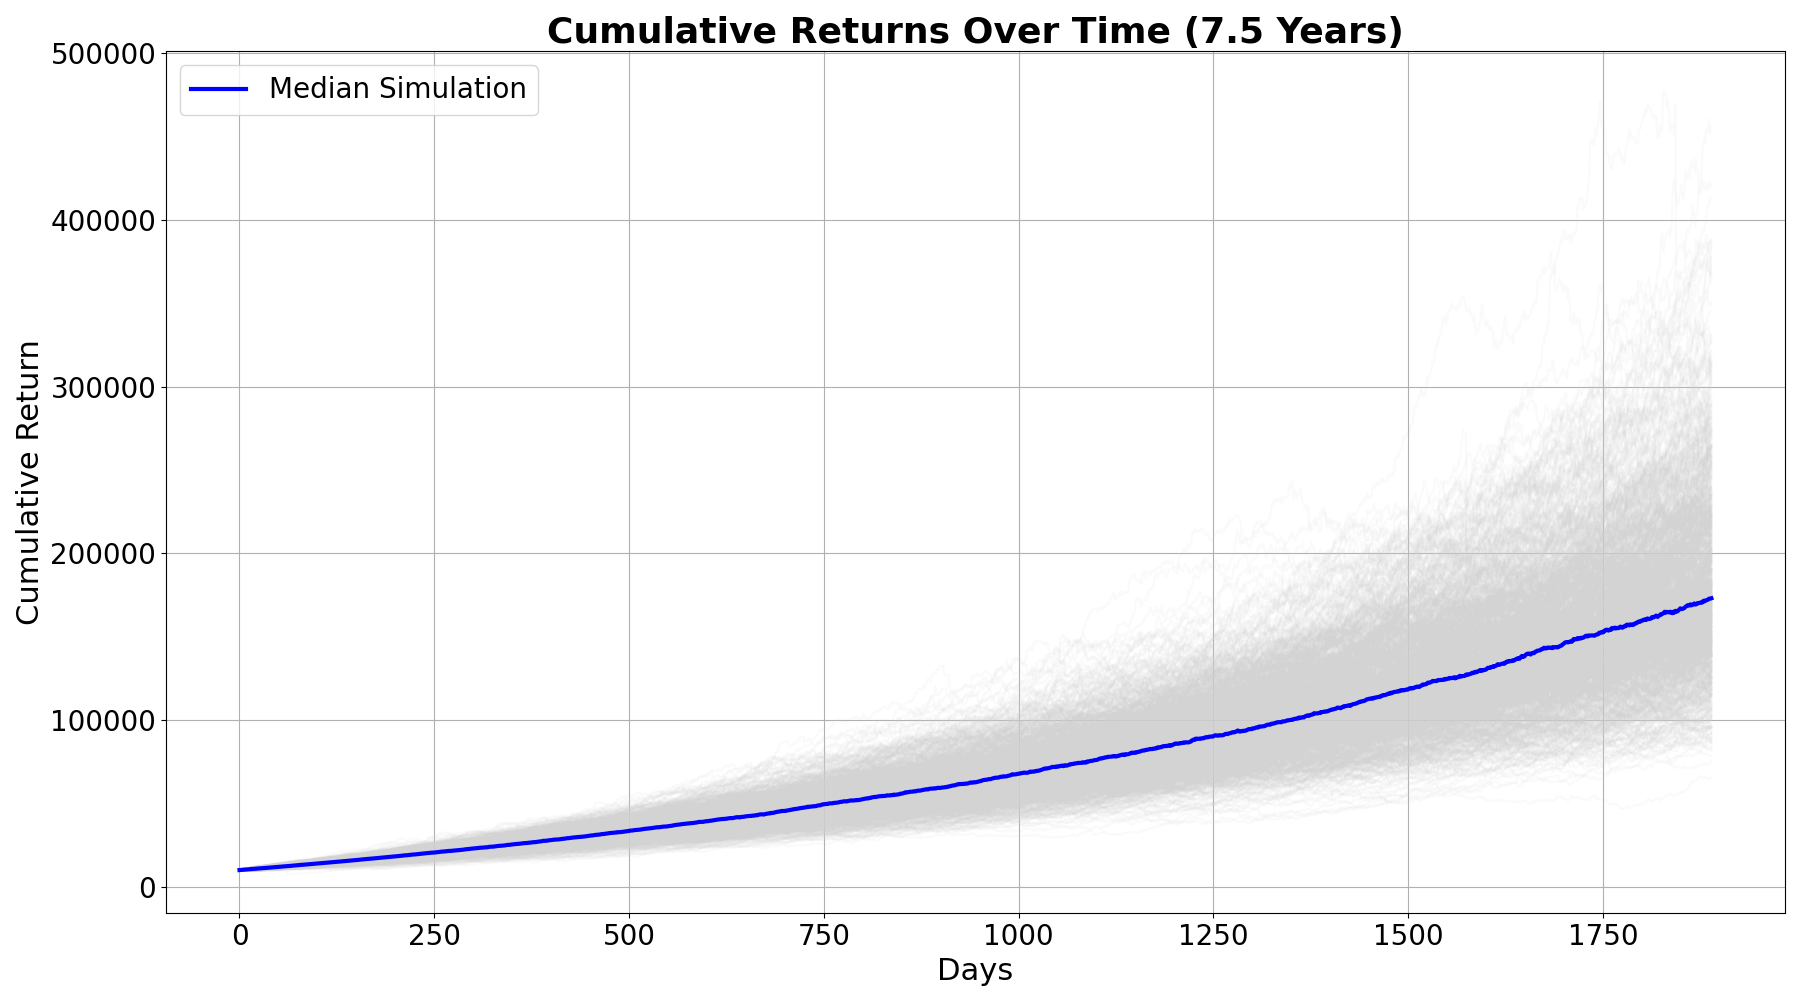
\includegraphics[width=0.8\textwidth]{../Figures/cumulative_returns_over_time_7_5_years.png}
    \caption{Cumulative Returns Over Time (7.5 Years)}
    \label{fig:cumulative_returns_7_5y}
\end{figure}

\textbf{Interpretation:} Figure \ref{fig:cumulative_returns_7_5y} illustrates the cumulative returns of the optimal portfolio over a 7.5-year period. This figure shows a smoother and more pronounced growth compared to the 5-year horizon, reflecting the benefits of an extended investment period.

\begin{figure}[!htbp]
    \centering
    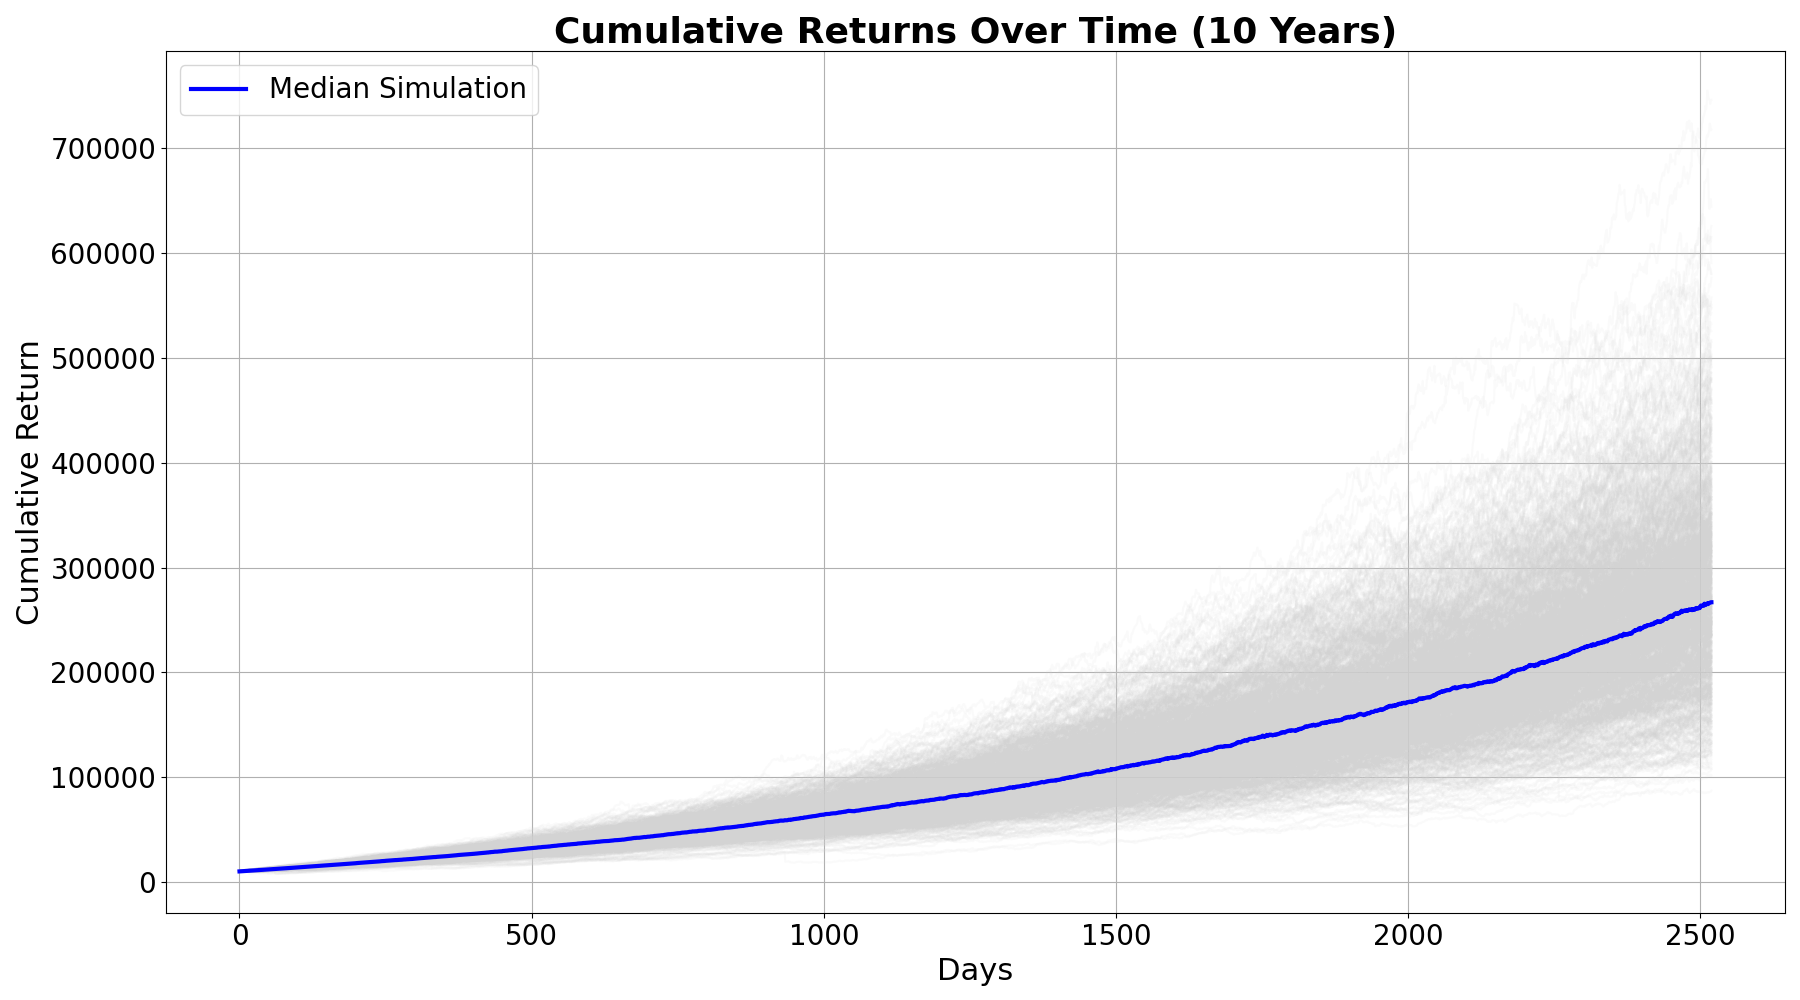
\includegraphics[width=0.8\textwidth]{../Figures/cumulative_returns_over_time_10_years.png}
    \caption{Cumulative Returns Over Time (10 Years)}
    \label{fig:cumulative_returns_10y}
\end{figure}

\textbf{Interpretation:} Figure \ref{fig:cumulative_returns_10y} depicts the cumulative returns over a 10-year period, showing the most stable and highest growth among the three horizons. This emphasizes the advantage of long-term investment strategies.







\subsection{Summary Statistics}
Summary statistics for the dataset are presented in Table \ref{tab:summary-stats}. These statistics were generated using the \texttt{../Data/summary\_stats.csv} file produced by the Python scripts.

\begin{table}[h!]
\centering
\scriptsize
\begin{tabular}{lccccccc}
\hline
Statistic & \begin{tabular}[c]{@{}c@{}}Mean Final \\ Portfolio Value (\$)\end{tabular} & \begin{tabular}[c]{@{}c@{}}Median Final \\ Portfolio Value (\$)\end{tabular} & \begin{tabular}[c]{@{}c@{}}10th Percentile Final \\ Portfolio Value (\$)\end{tabular} & \begin{tabular}[c]{@{}c@{}}90th Percentile Final \\ Portfolio Value (\$)\end{tabular} & \begin{tabular}[c]{@{}c@{}}Total Percentage \\ Yield (\%)\end{tabular} & \begin{tabular}[c]{@{}c@{}}Annual Percentage \\ Yield (\%)\end{tabular} \\
\hline
10-Year Horizon & 283094.44 & 265864.65 & 171232.59 & 420935.51 & 2730.94 & 39.70 \\
7.5-Year Horizon & 180745.35 & 173433.88 & 116972.91 & 256760.32 & 1707.45 & 47.10 \\
5-Year Horizon & 101559.42 & 98327.18 & 67062.20 & 139233.79 & 915.59 & 58.98 \\
\hline
\end{tabular}
\caption{Summary Statistics of the Dataset}
\label{tab:summary-stats}
\end{table}

\textbf{Interpretation:} Table \ref{tab:summary-stats} provides a detailed summary of the statistical outcomes for each investment horizon. The mean and median final portfolio values give insights into the expected performance, while the 10th and 90th percentile values offer a perspective on the range of potential outcomes. The total and annual percentage yields reflect the overall return potential of the portfolios over their respective horizons.

\newpage

